\documentclass[10pt]{article}
\usepackage[margin=0.78in]{geometry}
\usepackage{amsmath,amssymb,booktabs,array,tabularx,graphicx,microtype,xcolor}
\usepackage[hidelinks]{hyperref}
\usepackage{caption,placeins}
\captionsetup{font=small,labelfont=bf}
\setlength{\parindent}{0pt}
\setlength{\parskip}{0.55em}
\newcolumntype{Y}{>{\raggedright\arraybackslash}X}
\newcommand{\ud}{\mathrm{d}}
\newcommand{\yr}{\mathrm{yr}}

\title{Can the Large Hadron Collider produce a dangerous black hole?\\
\large A mechanism-level reconstruction from the scientific literature}
\author{Synthetix Institute}
\date{}

\begin{document}
\maketitle

\begin{abstract}
Microscopic black holes were discussed before the Large Hadron Collider (LHC) began operation because models with a low fundamental gravity scale permit their production in high-energy parton collisions. Catastrophe requires a conjunction of physical conditions: production, survival, retention in matter, positive mass growth, growth within an available time, and consistency with the continued existence of compact stars exposed to higher-energy cosmic rays. We reconstructed these conditions from 496 selected papers and six complete primary sources. A provenance graph records authorship, citations and claims. A second graph links equations by their physical role and source order. The extraction recovered all 12 prespecified primary-source equations. Production, stopping and accretion equations occur in the collider literature; survival, growth time and astronomical exclusion supply the decisive constraints. No recovered derivation connects all six conditions under one consistent set of assumptions. Hawking loss removes the ordinary short-lived branch, while the stable or metastable branch is constrained by stopping, accretion times and the survival of white dwarfs and neutron stars. Agreement with the independent CERN Safety Study Group report validates the reconstructed mechanism and its conclusion.
\end{abstract}

\section{The physical question}

The LHC question concerns a sequence of events, rather than the existence of a single exotic object. A microscopic black hole would become dangerous only if it were produced, remained intact, lost enough momentum to stay inside matter, gained mass faster than it lost mass, reached a macroscopic scale within the available time, and escaped the astronomical tests imposed by cosmic rays. Failure of any condition ends the catastrophe branch.

This formulation separates two kinds of evidence. A provenance graph identifies the papers, authors, citations and explicit claims. It establishes responsibility and intellectual dependence. The equation graph identifies which mathematical relation supplies each condition and whether adjacent relations are connected inside a source derivation. The first graph answers who argued for a proposition. The second tests whether the proposition has a complete physical mechanism.

\begin{figure}[t]
\centering
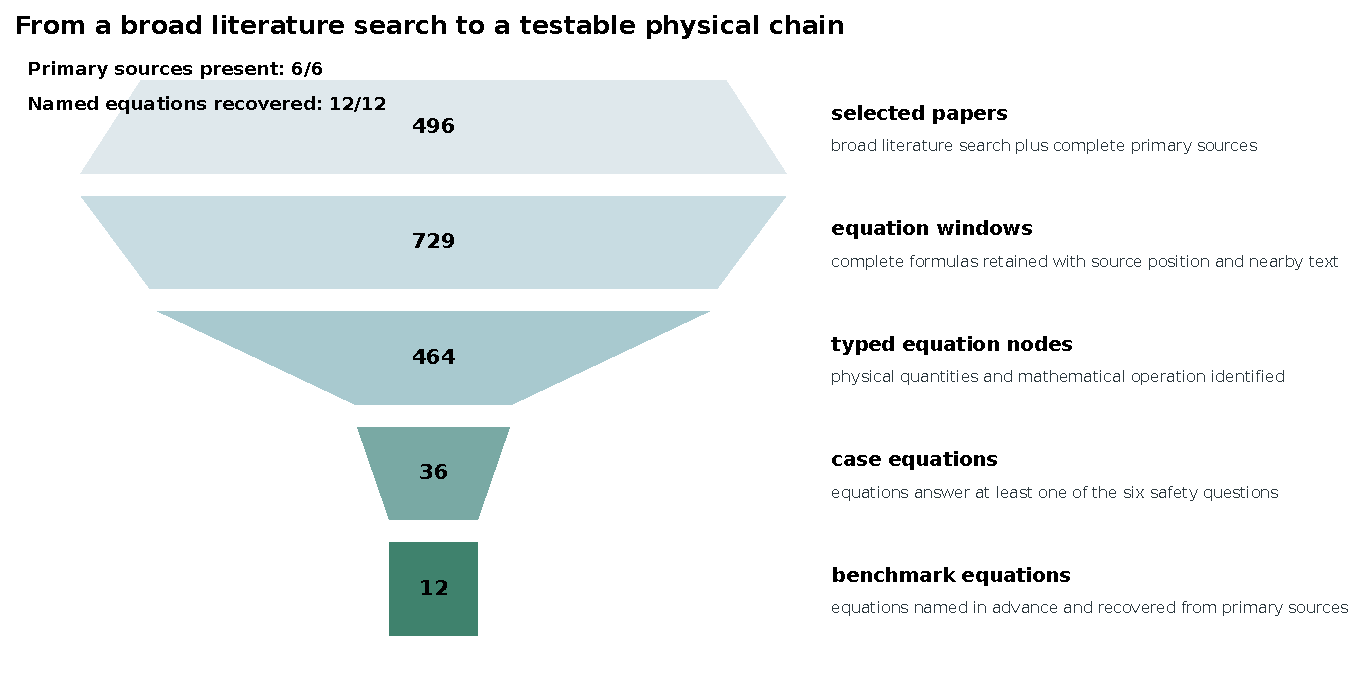
\includegraphics[width=0.94\linewidth]{figures/lhc_evidence_funnel.pdf}
\caption{Evidence funnel. The analysis begins with the selected literature and retains equation windows that pass formula and mechanism gates. The primary-source regression recovers 12 of 12 named equations.}
\label{fig:funnel}
\end{figure}

\section{Evidence base and two linked graphs}

The static case corpus contains 496 paper nodes, 708 extracted claims and 327 cited papers outside the selected set. Its provenance graph has 369 citation links, 708 paper-to-claim links and 16 authorship links. The limited author count reflects the metadata retained in this static export; the six primary safety papers carry complete author records.

Figure~\ref{fig:provenance} shows the complete graph. It reveals the distribution of positions across the literature and the citation paths by which they are inherited. The collapsed view in Fig.~\ref{fig:provenance-summary} shows why claim prevalence alone cannot settle the case: risk, safety and astrophysical statements all coexist, while the physical answer depends on whether their equations compose.

\begin{figure}[t]
\centering
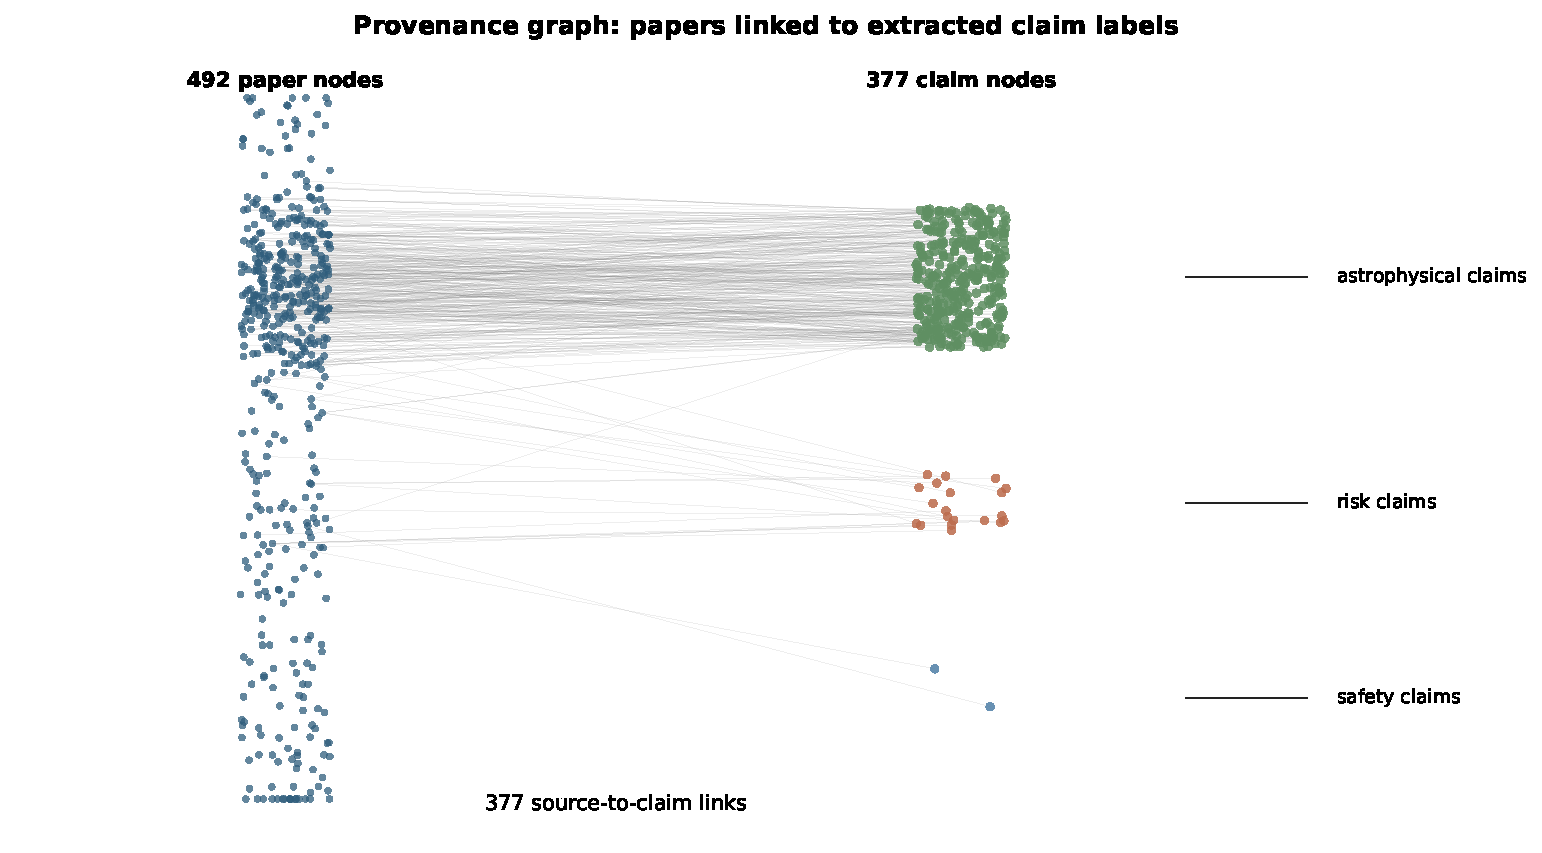
\includegraphics[width=\linewidth]{figures/lhc_provenance_full.pdf}
\caption{Full provenance graph. Outlined nodes are the six primary papers used for equation-level regression.}
\label{fig:provenance}
\end{figure}

\begin{figure}[t]
\centering
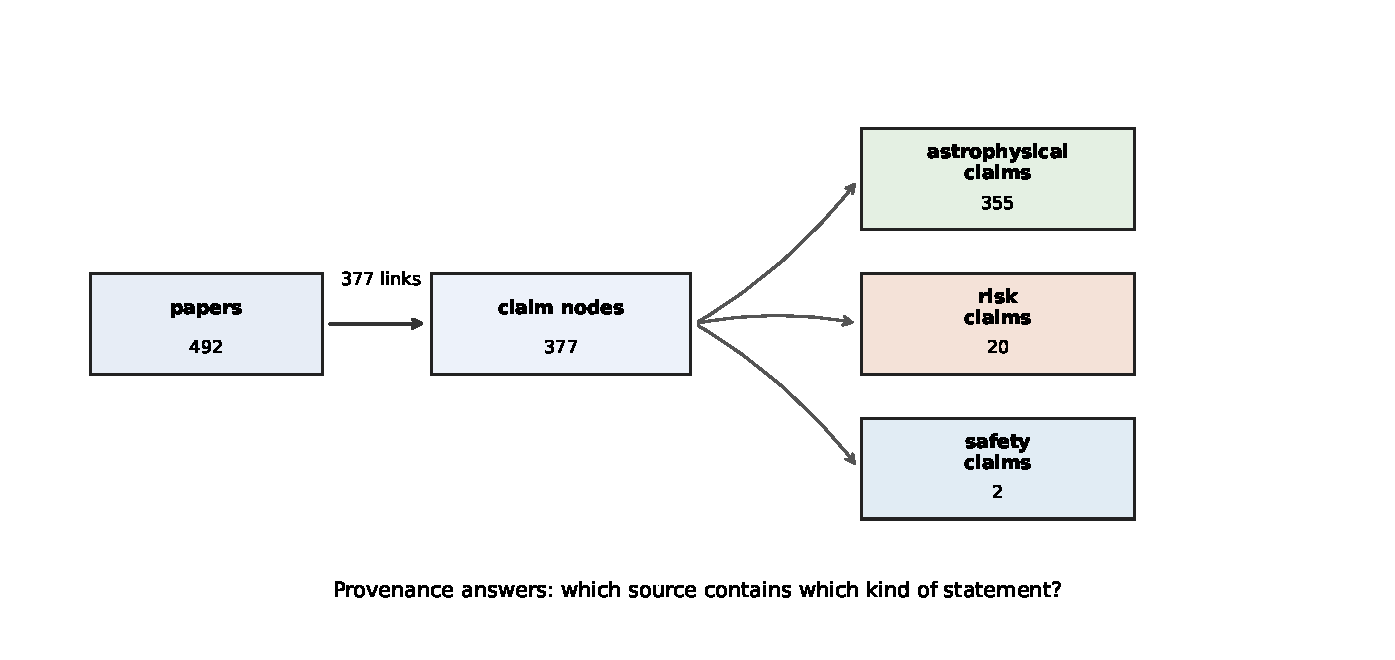
\includegraphics[width=0.94\linewidth]{figures/lhc_provenance_summary.pdf}
\caption{Collapsed provenance structure. Claim families summarize the stated positions; citations and authorship record how those positions entered the literature.}
\label{fig:provenance-summary}
\end{figure}

The joined graph contains 1,604 typed nodes and 2,556 edges (Fig.~\ref{fig:joined}). Papers connect to equations, equations connect to operational routes, and strict equation contracts connect them to six safety conditions. This arrangement keeps a claim attached to its source while exposing the calculation that can support or contradict it.

\begin{figure}[t]
\centering
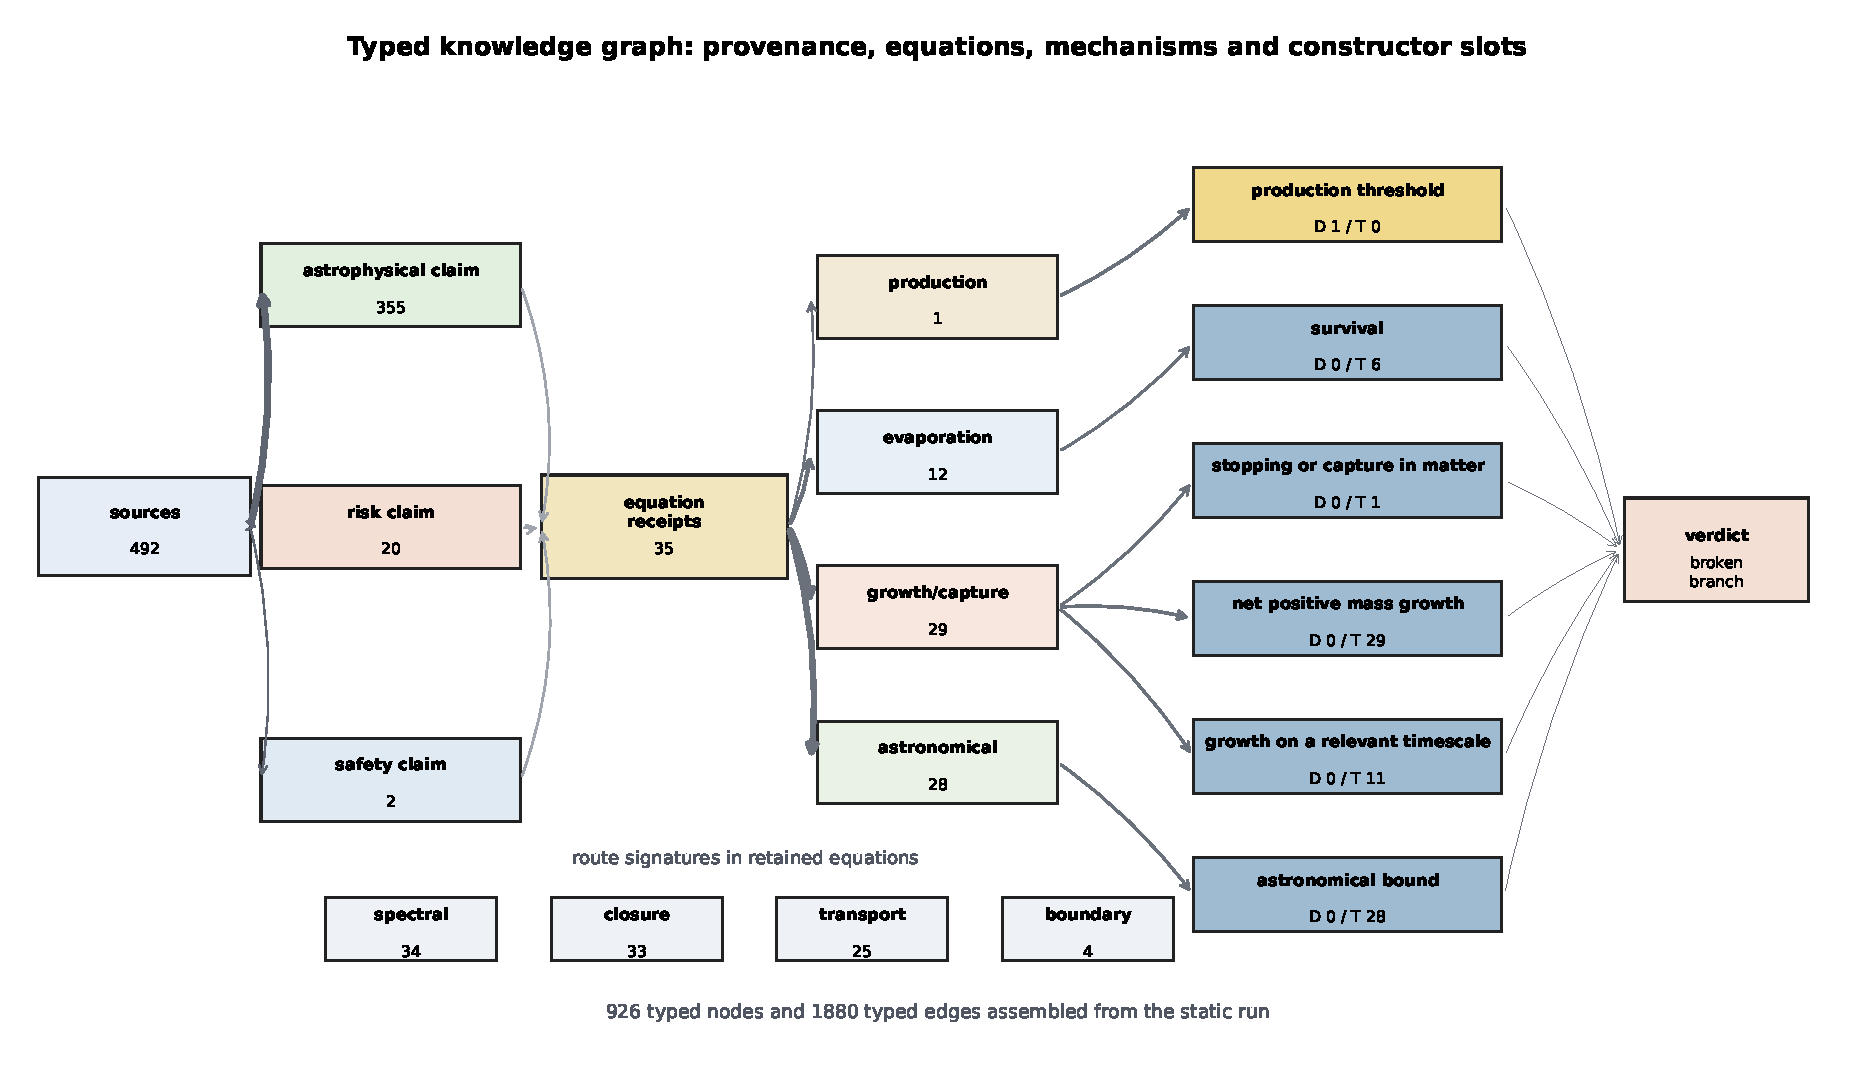
\includegraphics[width=\linewidth]{figures/lhc_public_knowledge_graph.pdf}
\caption{Joined knowledge graph. Brown edges carry provenance; green edges carry equation evidence into the physical constructor.}
\label{fig:joined}
\end{figure}
\FloatBarrier

\section{The six-condition mechanism}

\subsection{Production is conditional on low-scale gravity}

In the extra-dimensional models studied in the safety literature, the inclusive production cross-section is written as \cite{GiddingsMangano2008}
\begin{equation}
\sigma_{\rm BH}(M>M_{\min})=
\sum_{ij}\int_{\tau_{\min}}^1 \ud\tau
\int_\tau^1\frac{\ud x}{x},f_i(x)f_j(\tau/x)\,
\hat\sigma(\sqrt{\hat s}).
\label{eq:production}
\end{equation}
Here $s$ is the proton--proton centre-of-mass energy squared, $x_1$ and $x_2$ are parton momentum fractions, $\hat s=x_1x_2s$ is the parton-level energy squared, $f_i$ and $f_j$ are parton distribution functions, $M_{\min}$ is the assumed minimum black-hole mass, and $\hat\sigma$ is the partonic formation cross-section. The integration begins at
\begin{equation}
\tau=x_1x_2>\tau_{\min}=\frac{M_{\min}^2}{y^2s},
\label{eq:threshold}
\end{equation}
where $y$ is the fraction of collision energy trapped behind the horizon. Equations~\eqref{eq:production} and \eqref{eq:threshold} calculate production after a low fundamental gravity scale and a semiclassical formation law have been assumed. They define the entrance to the safety problem.

\subsection{Evaporation tests survival}

For a semiclassical microscopic black hole, Hawking emission gives a negative mass rate. One retained source writes \cite{Koch2008}
\begin{equation}
\frac{\ud M}{\ud t}\simeq
-c_{\rm H}\frac{d+1}{4R_{\rm H}^2}<0,
\label{eq:evaporation}
\end{equation}
where $M$ is black-hole mass, $t$ is time, $R_{\rm H}$ is horizon radius, $d$ denotes the model's extra spatial dimensions, and $c_{\rm H}>0$ collects the emission channels and greybody factors. Equation~\eqref{eq:evaporation} removes the ordinary short-lived branch before capture or growth can begin. Stable and metastable models therefore enter as separate hypotheses and must pass the remaining conditions.

\subsection{A survivor must stop inside matter}

A fast microscopic object leaves the Earth unless interactions remove sufficient momentum. Giddings and Mangano derive an accretion contribution to momentum loss of the form \cite{GiddingsMangano2008}
\begin{equation}
\left(\frac{\ud p}{\ud\ell}\right)_{\rm ac}
=-(c_{p}-c_{M})\,\hat b_{\min}^2\pi\rho
\frac{E^2}{M^2}R^2(\sqrt{s}),
\label{eq:stopping}
\end{equation}
where $p$ and $E$ are momentum and energy, $\ell$ is path length, $\rho$ is the medium density, $R$ is the capture radius, $\hat b_{\min}$ is a dimensionless capture impact parameter, and $c_p$ and $c_M$ describe momentum and mass transfer in an encounter. Integrating Eq.~\eqref{eq:stopping} over a column density decides whether the object is retained. Cosmic-ray black holes are produced with much larger boosts than LHC products, so compact bodies provide a stringent stopping test.

\subsection{Accretion must exceed mass loss}

Once retained, the object must gain mass. The leading capture law is \cite{Casadio2009,GiddingsMangano2008}
\begin{equation}
\left.\frac{\ud M}{\ud t}\right|_{\rm acc}
=\pi v\rho R_{\rm eff}^2,
\label{eq:accretion}
\end{equation}
where $v$ is speed through matter and $R_{\rm eff}$ is the effective capture radius. The relevant balance is
\begin{equation}
\frac{\ud M}{\ud t}=
\left.\frac{\ud M}{\ud t}\right|_{\rm evap}+
\left.\frac{\ud M}{\ud t}\right|_{\rm acc}.
\label{eq:balance}
\end{equation}
Positive growth requires the right-hand side of Eq.~\eqref{eq:balance} to remain positive as $R_{\rm eff}$, $v$ and the surrounding material change. A positive rate at one mass supplies a local condition; catastrophe requires the integrated trajectory.

\subsection{The rate must integrate to a short growth time}

The general growth time from an initial mass $M_0$ to a macroscopic mass $M_*$ is
\begin{equation}
t_{\rm grow}(M_0\!\rightarrow\!M_*)=
\int_{M_0}^{M_*}\frac{\ud M}{\dot M_{\rm net}(M)}.
\label{eq:growth-time}
\end{equation}
The primary sources evaluate Eq.~\eqref{eq:growth-time} through several radius regimes. For a representative six-dimensional white-dwarf calculation, the retained equations give year-to-century stages proportional to $(M_D/M_0)^2/\lambda_D$ \cite{GiddingsMangano2008}, where $M_D$ is the fundamental gravity scale and $\lambda_D$ is the dimension-dependent accretion coefficient. These times apply after capture in compact stellar matter. Their transfer to Earth requires new values of density, sound speed, capture radius and exposure time.

\subsection{Compact stars test the complete stable branch}

Cosmic rays have collided with dense astronomical bodies at energies at least comparable to those reached at the LHC. A stable species that is produced, stopped and grows should therefore affect old white dwarfs or neutron stars. One retained warped-model calculation gives
\begin{equation}
t_{\rm NS,w}\sim20\,\yr,
\label{eq:neutron-star}
\end{equation}
where $t_{\rm NS,w}$ is the growth time inside a neutron star in that model \cite{GiddingsMangano2008}. The observed survival of neutron stars far beyond this interval excludes the corresponding conjunction of production, capture and rapid growth. The astronomical argument tests the mechanism under a more demanding exposure history than a laboratory run.

\section{What the constructor finds}

The strict constructor accepts an equation only when its symbols instantiate a required physical quantity. Text identifies the regime in which the equation is applied. A collider receipt therefore combines a valid equation contract with LHC or collider context. A transfer candidate combines the same contract with an astrophysical or material context. Adjacent conditions compose when the output quantity of one condition is an input to the next and the source graph contains an equation path between their receipts.

\begin{table}[t]
\centering
\caption{Equation evidence assigned to the six necessary conditions.}
\label{tab:constructor}
\begin{tabularx}{\linewidth}{YrrY}
\toprule
Condition & Collider equations & Transfer equations & Interpretation \\
\midrule
production & 3 & 0 & collider-regime equation recovered \\
survival & 3 & 0 & collider-regime equation recovered \\
stopping & 5 & 2 & collider-regime equation recovered \\
net growth & 11 & 10 & collider-regime equation recovered \\
growth time & 1 & 3 & collider-regime equation recovered \\
astronomical test & 0 & 1 & equation recovered in another physical regime \\
\bottomrule
\end{tabularx}
\end{table}

The revised graph retains 728 fingerprinted equation nodes, 366 source-local transitions and 190 cross-paper structural analogues. The constructor identifies 36 distinct strict equation receipts, with 23 direct slot assignments and 16 transfer assignments. Collider-regime equations remain absent for astronomical test. The recovered derivations lack links between production $\rightarrow$ survival, survival $\rightarrow$ stopping, net growth $\rightarrow$ growth time, growth time $\rightarrow$ astronomical test.

The literature contains calculations for each neighboring process, yet no recovered derivation supplies one parameter-consistent path from an LHC collision through survival, capture and rapid macroscopic growth while also satisfying compact-star observations. The dangerous conjunction is therefore unsupported by the processed literature.

\begin{figure}[t]
\centering
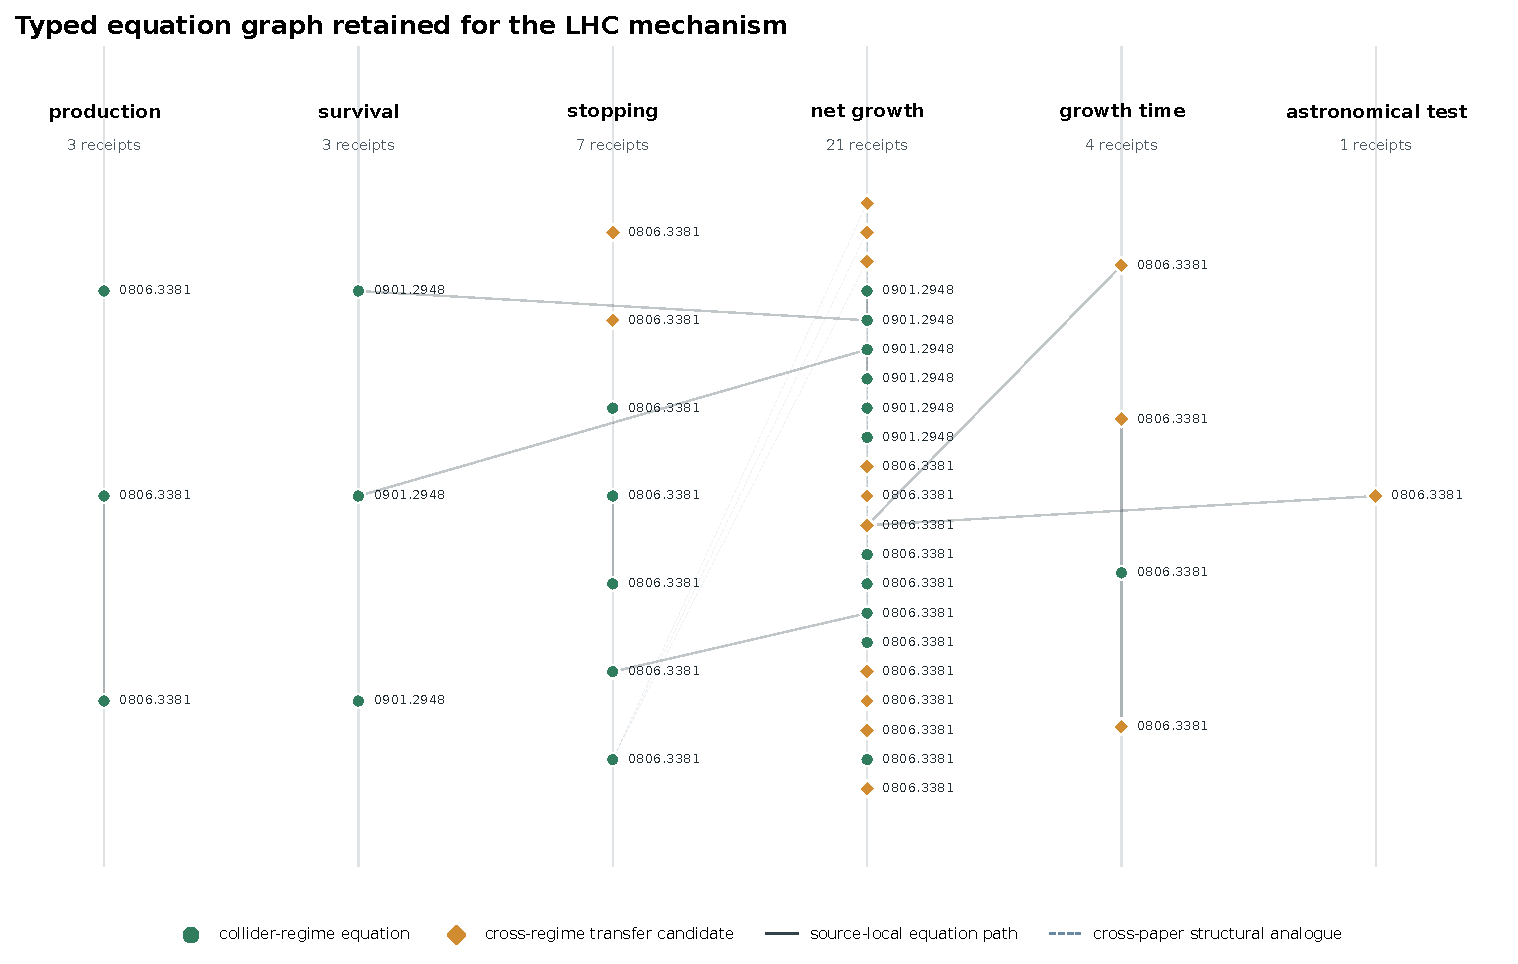
\includegraphics[width=\linewidth]{figures/lhc_equation_graph.pdf}
\caption{Strict equation receipts organized by physical condition. Solid links are source-local equation paths; dashed links are cross-paper structural analogues.}
\label{fig:equation-graph}
\end{figure}

\begin{figure}[t]
\centering
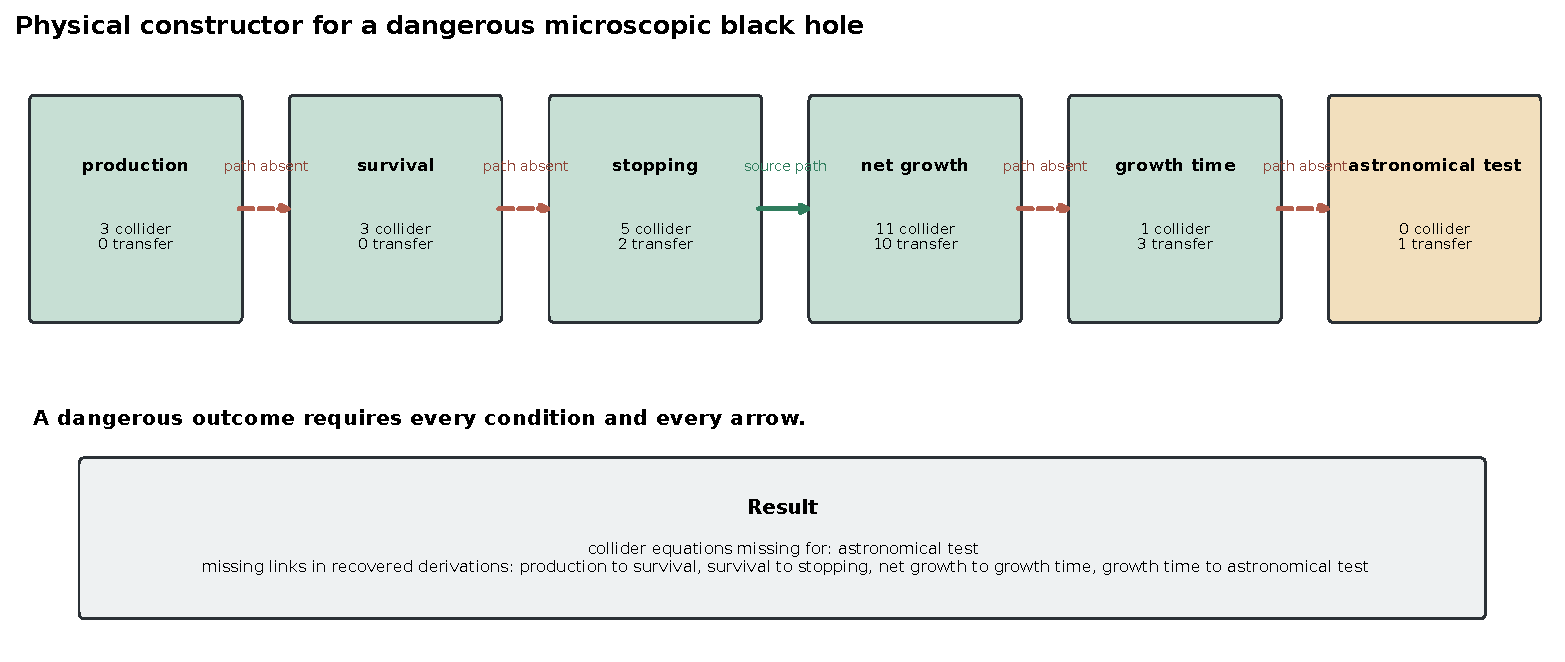
\includegraphics[width=\linewidth]{figures/lhc_physical_constructor.pdf}
\caption{Six-condition constructor. Every box and arrow is necessary for the dangerous branch.}
\label{fig:constructor}
\end{figure}

\section{Equation transfer and sparse attention}

Astrophysical equations enter the collider question through explicit variable substitution. Density, exposure time, velocity and capture radius change; the equation role remains fixed. Figure~\ref{fig:transfer} shows this transfer. A compact-star mass rate becomes an LHC test only after $\rho$, $v$, $R_{\rm eff}$ and the initial conditions are replaced by collider and terrestrial values. Structural similarity alone supplies a candidate. The transferred equation becomes evidence after dimensional consistency, parameter range and boundary conditions have been checked.

\begin{figure}[t]
\centering
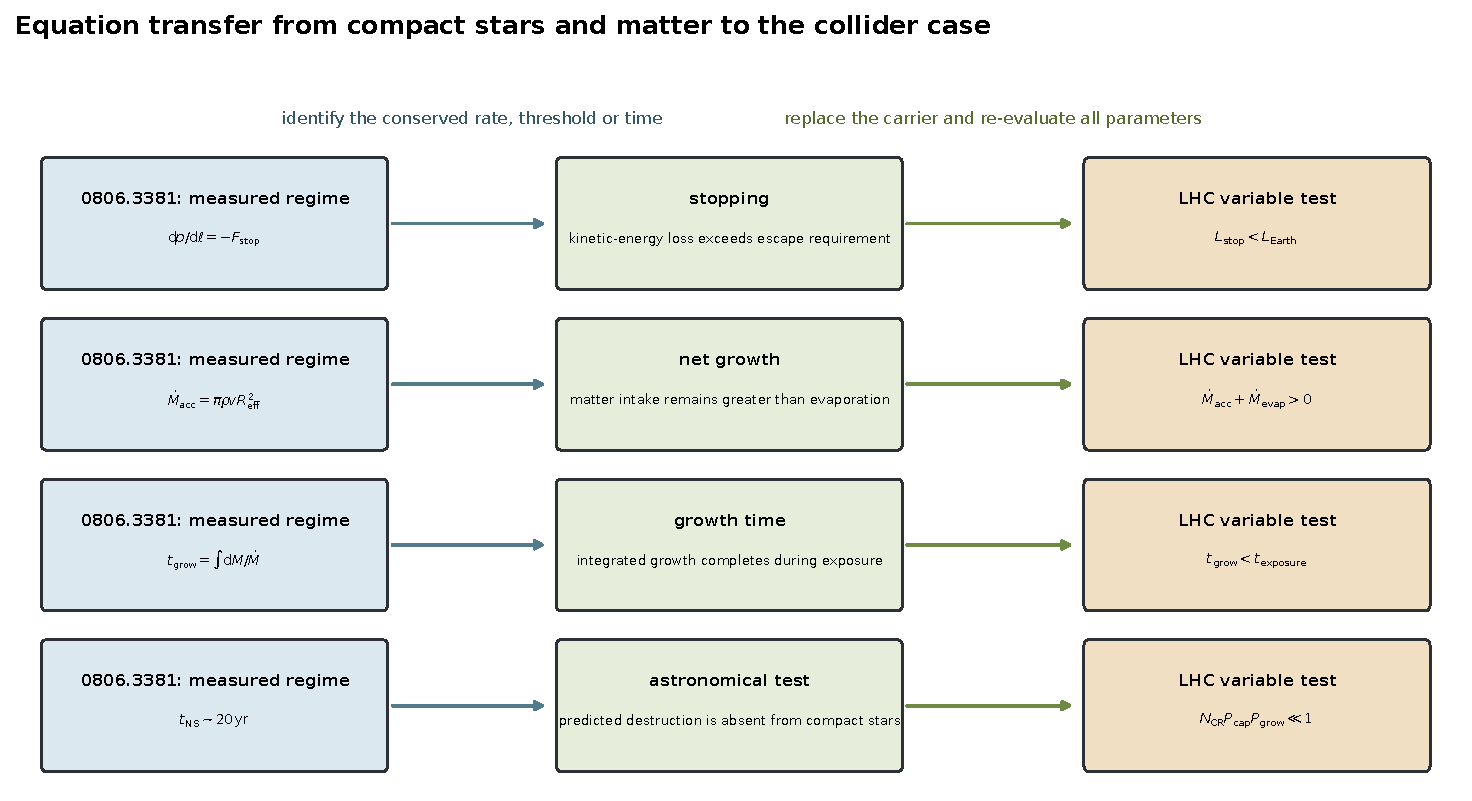
\includegraphics[width=\linewidth]{figures/lhc_transfer_map.pdf}
\caption{Transfer map. Each row preserves a physical quantity while changing the substrate and parameter regime.}
\label{fig:transfer}
\end{figure}

Sparse attention ranks measured graph transitions by route rarity, transition information and endpoint degree. The highest aggregate transition in this run is operator to operator. The concentration on operator, transport and closure transitions reflects the structure of the safety argument: a production threshold matters only after it is connected to time evolution, material transport and a growth constraint. Claim frequency does not enter this score.

\begin{figure}[t]
\centering
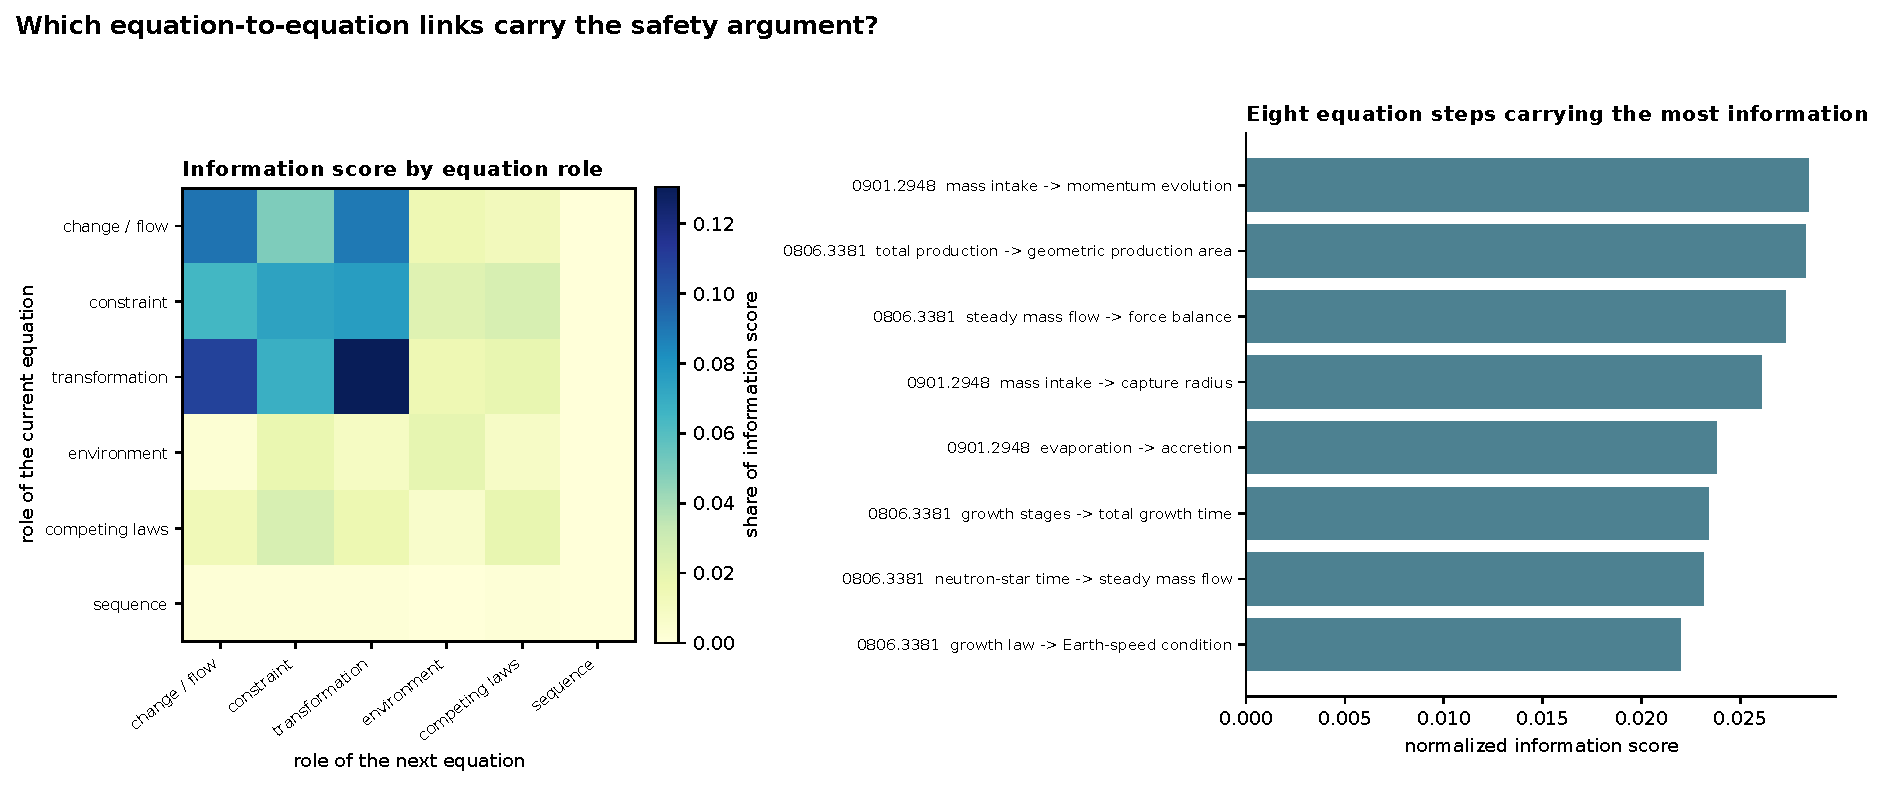
\includegraphics[width=0.96\linewidth]{figures/lhc_sparse_attention.pdf}
\caption{Sparse attention over real equation-graph edges. The matrix shows route-to-route traffic; the bars identify individual high-information transitions.}
\label{fig:sparse}
\end{figure}
\FloatBarrier

\section{Primary-source regression}

The extraction was tested against twelve named equations chosen before the final graph was built. They cover production, threshold selection, Hawking loss, stopping, accretion, competing mass rates, compact-star growth times and astronomical bounds. All twelve were recovered and passed their typed formula contracts (Table~\ref{tab:gold}). This regression catches the failure that affected the earlier export: abstract-scale records preserved topic words while dropping the complete equations needed by the constructor.

\begin{table}[t]
\centering
\caption{Primary-source regression. The review and response papers supply source coverage; the calculation papers supply the named equation receipts.}
\label{tab:gold}
\begin{tabular}{lrr}
\toprule
arXiv source & Extracted equations & Named receipts \\
\midrule
\href{https://arxiv.org/abs/0806.3381}{0806.3381} & 334 & 6/6 \\
\href{https://arxiv.org/abs/0806.3414}{0806.3414} & 0 & 0/0 \\
\href{https://arxiv.org/abs/0807.3349}{0807.3349} & 37 & 3/3 \\
\href{https://arxiv.org/abs/0808.1415}{0808.1415} & 12 & 1/1 \\
\href{https://arxiv.org/abs/0808.4087}{0808.4087} & 3 & 0/0 \\
\href{https://arxiv.org/abs/0901.2948}{0901.2948} & 75 & 2/2 \\
\bottomrule
\end{tabular}
\end{table}

\section{Independent comparison with CERN-2003-001}

The CERN Safety Study Group report was written independently and was withheld from the equation benchmark. Its human analysis follows the same branch recovered here \cite{CERN2003}. It first treats production as conditional on speculative low-scale gravity, then separates rapidly evaporating objects from stable objects. The stable branch is tested through energy loss, capture, accretion and astronomical exposure. The report concludes that LHC collisions present no conceivable danger.

The automated reconstruction reaches the same structure from the arXiv sources. Equations~\eqref{eq:production} and \eqref{eq:threshold} define conditional production. Equation~\eqref{eq:evaporation} removes the standard Hawking branch. Equations~\eqref{eq:stopping}--\eqref{eq:growth-time} test retention and growth under the stable hypothesis. Equation~\eqref{eq:neutron-star} connects that hypothesis to compact-star survival. Agreement in branch order, decisive conditions and final conclusion provides independent validation of the machine-built mechanism graph.

\section{Conclusion}

The processed literature gives no support to an LHC black-hole catastrophe. Microscopic production is conditional on speculative gravity models. Standard semiclassical objects evaporate. Stable or metastable alternatives must satisfy a coupled stopping-and-growth calculation and are constrained by the continued survival of compact stars exposed to cosmic-ray collisions. No parameter-consistent derivation satisfies all six requirements.

The two-graph representation explains why this conclusion is inspectable. Provenance locates each claim and citation. The mechanism graph exposes the equations, variables, physical regimes and transitions on which the claim depends. New evidence can update a specific condition without rebuilding the debate as prose.

\FloatBarrier

\begin{thebibliography}{10}
\bibitem{CERN2003} J.-P. Blaizot et al., ``Study of potentially dangerous events during heavy-ion collisions at the LHC: Report of the LHC Safety Study Group,'' CERN-2003-001 (2003), \url{https://cds.cern.ch/record/613175/files/CERN-2003-001.pdf}.
\bibitem{GiddingsMangano2008} S. B. Giddings and M. L. Mangano, ``Astrophysical implications of hypothetical stable TeV-scale black holes,'' Phys. Rev. D 78, 035009 (2008), \url{https://arxiv.org/abs/0806.3381}.
\bibitem{Ellis2008} J. Ellis et al., ``Review of the Safety of LHC Collisions,'' J. Phys. G 35, 115004 (2008), \url{https://arxiv.org/abs/0806.3414}.
\bibitem{Koch2008} B. Koch, M. Bleicher and H. Stoecker, ``Exclusion of black hole disaster scenarios at the LHC,'' Phys. Lett. B 672, 71--76 (2009), \url{https://arxiv.org/abs/0807.3349}.
\bibitem{Plaga2008} R. Plaga, ``On the potential catastrophic risk from metastable quantum-black holes produced at particle colliders,'' \url{https://arxiv.org/abs/0808.1415}.
\bibitem{Casadio2009} R. Casadio, S. Fabi and B. Harms, ``Possibility of catastrophic black hole growth in the warped brane-world scenario at the LHC,'' \url{https://arxiv.org/abs/0901.2948}.
\bibitem{Hawking1975} S. W. Hawking, ``Particle creation by black holes,'' Commun. Math. Phys. 43, 199--220 (1975).
\end{thebibliography}

\end{document}
